%======================================================================
\chapter{Verification and Application}
%======================================================================
In this chapter, two-dimensional \acrshort{dem} models are used to demonstrate the effectiveness of the up-scaling methodology. The framework is validated using three tests: 1) The homogenized stress and strain behaviour obtained from the \acrshort{dem} microscale response are compared to that of the macroscale response. This test verifies the effectiveness of the parameter estimation module and the ability of the chosen macroscale constitutive model to capture the salient features of \acrshort{nfr} behaviour. 2) The homogenization and parameter estimation algorithms are rerun using the same data, but with different \acrshort{rev} sizes to investigate the \acrshort{rev} size effect has on the resultant parameter set. 3) Slope stability analyses carried out by both \acrfull{dns} with a \acrshort{dem} model and with an up-scaled macroscale model are compared. This last test verifies the whole up-scaling methodology.

The up-scaling is conducted by running a series of four quasi-static \acrshort{dem} virtual 'triaxial' compression tests under different confining stresses. These are not true triaxial tests as simulations are in 2D, but illustrate the method regardless. Algorithms are rerexecuted using different \acrshort{rev} sizes to determine an appropriate \acrshort{rev} size. In a macroscopically homogenous domain, as the \acrshort{rev} size increases, the parameter values will converge to a single value, when the \acrshort{rev} is too small, local heterogeneities induce a variance into the optimal parameter set.

%----------------------------------------------------------------------
\section{DEM Simulations}
%----------------------------------------------------------------------

The \acrshort{dem} models used consist of a pseudo-random isotropic fracture network defined by a Voronoi tessellation. The average block size is specified to be 0.5m using 20 iterations of Lloyd's method \citep{Lloyd_1982} in order to achieve an even size distribution. A 10m x 10m domain was determined to be sufficiently large to represent the rock mass behaviour as an \acrshort{rev}. 

A Mohr-Coulomb plasticity model was used as the constitutive model to describe the plastic behaviour of the intact  (deformable blocks) and the joint (natural fracture) behaviour was governed by a Coulomb area slip model. The parameters for the rock and joints summarized in Table \ref{tab:demProp} are representative of a fractured granitic rock mass. The joints are relatively weak compared to the blocks, so the blocks behave mostly elastically. 

\begin{table}[!htb]
\centering
\caption{{Rock and joint properties for DEM Simulations}}
\label{tab:demProp}
\begin{tabularx}{\textwidth}{@{}YYY@{}}
\toprule
\textbf{Property Type} & \textbf{Property} & \textbf{Value} \\ \midrule
\multirow{7}{*}{Rock}  & Young's Modulus   & $65 GPa$       \\
                       & Poisson's Ratio   & $0.2$          \\
                       & Density           & $2.7 g/cm^3$   \\
                       & Friction Angle    & $51^{\circ}$   \\
                       & DilationAngle     & $0^{\circ}$    \\
                       & Cohesion          & $55.1 MPa$     \\
                       & Tensile Strength  & $11.7 MPa$     \\ \cmidrule(r){1-1}
\multirow{6}{*}{Joint} & Friction Angle    & $32^{\circ}$   \\
                       & Dilation Angle    & $5^{\circ}$    \\
                       & Cohesion          & $100 kPa$      \\
                       & Tensile Strength  & $100 kPa$      \\
                       & Normal Stiffness  & $10 GPa/m$     \\
                       & Shear Stiffness   & $1 GPa/m$      \\ \bottomrule
\end{tabularx}

\end{table}

The blocks are meshed with linear three-node triangular plane strain finite difference elements with an average side length of 0.5m. This discretization yielded 5-10 zones within each block. A rounding length of 10\% of the average block edge length (0.05m) is applied to the blocks to prevent numerical instabilities in the contact algorithm. Quasi-static analysis is obtained through dynamic relaxation, in which the dynamic equations are integrated in time using velocity-proportional viscous damping and mass scaling. State data of the model is collected at 50 evenly spaced intervals. 

The quasi-static loading of the \acrshort{dem} simulations is intended to imitate triaxial laboratory tests, so a constant confining stress was applied on the lateral boundaries of the \acrshort{dem} model. Loading is achieved by applying vertical displacements to the top boundary while fixing the bottom boundary, compressing the model to a vertical strain of $5\%$ for four confining horizontal stresses: $0.5MPa$, $1MPa$, $2MPa$, and $4MPa$. These load paths capture key physical phenomena including the pressure dependent yield of the \acrshort{nfr}, hardening, and the dependence of damage initiation on the triaxiality. 

%Second, triaxial compressive strength test at a strain rate of $0.05\%/s$ for $50s$ followed by a tensile strain rate of $0.05\%/s$ for $50s$ to observe the stiffness degradation and elastic recovery response of the \acrshort{dem} simulations during unloading. Here, even though the extended Drucker-Prager model is formulated for monotonic loading, the cyclic loading capacity of this model was investigated. The idea with these simulations was to strain the model past the yield point in order to investigate the post-yield behavior, but not strain the model to failure such that it loses all of its strength.

%----------------------------------------------------------------------
\section{Verification of the Parameter Estimation Module}
%----------------------------------------------------------------------

Using a \acrshort{pso} algorithm followed by an \acrshort{lma} optimization, the Drucker-Prager plasticity model with ductile damage is then fitted to the homogenized \acrshort{dem} simulation data in order to obtain an optimal parameter set. Each simulation is fit to 50 points defining the homogenized stress-strain curve resulting in a total of 200 data points for all four \acrshort{dem} simulations at different confining stresses. The \acrshort{pso} algorithm uses a swarm size of 24 for 100 generations which is found to be sufficient to converge to a consistent solution. 

Here, the \acrshort{cdm} model is confined laterally by the homogenized horizontal \acrshort{dem} stress and vertical displacements are prescribed by the homogenized vertical \acrshort{dem} strain with the parameter estimation algorithms programmed to match the horizontal strain and the vertical stress. Because of the large variation in observation magnitudes (between stress/strain and from different confining stresses), each curve is weighted with a normalization factor to prevent the large stress values from dominating parameter estimation. In addition, a linear weighting scheme is applied to each curve to give larger influence to the loading section and lesser influence to the post-damage section.

Parameter bounding limits are required by the optimization algorithms in order to limit the search space. These limits are chosen based on two criteria: physical limitations and numerical stability. If there exist physical limitations that prevent parameters from exceeding certain values or if there exists a range of realistic values that the parameter should not deviate from, then those physical limitations are specified as the bounds. In other cases, the parameter bounds come from numerical limitations such that beyond a certain capacity, certain parameter values would cause the simulations to become unstable. In these cases, a combination of the two bounding methods is used. The specified bounding limits for each parameter results can be seen in Table \ref{tab:paramDrucker}.

\begin{table}[!htb]
\centering
\caption{{Parameter estimation results for Drucker-Prager model with ductile damage}}
\label{tab:paramDrucker}
\begin{tabulary}{\textwidth}{@{}cCcCCC@{}}
\toprule
\textbf{Parameter}                 & \textbf{Symbol}                  & \textbf{Units} & \textbf{Lower Bound} & \textbf{Upper Bound} & \textbf{Optimum} \\ \midrule
Young's Modulus                    & $E$                              & $GPa$          & $1$                                                             & $25$                                                            & $1.8$                                                             \\
Poisson's Ratio                    & $\nu$                            &                & $0.1$                                                           & $0.4$                                                           & $0.15$                                                            \\
Dilation Angle                     & $\psi$                           & $^{\circ}$     & $5$                                                             & $15$                                                            & $22$                                                              \\
Flow Stress Ratio                  & $K$                              &                & $0.78$                                                          & $1$                                                             & $0.81$                                                            \\
Friction Angle                     & $\beta$                          & $^{\circ}$     & $45$                                                            & $60$                                                            & $56$                                                              \\
Initial Compressive Yield Strength & $\sigma_c^{iy}$                  & $kPa$          & $1$                                                             & $100$                                                           & $52$                                                              \\
Peak Compressive Yield Strength    & $\sigma_c^{p}$                   & $MPa$          & $0.5$                                                           & $5$                                                             & $3.1$                                                             \\
Strain at Peak Compressive Yield   & $\epsilon_c^{p}$                 & $\%$           & $0.5$                                                           & $5$                                                             & $1.7$                                                             \\
Yield Strain at -0.5 Triaxiality   & $\bar{\epsilon}^{pl}_{f_{-0.5}}$ & $\%$           & $0.01$                                                          & $0.1$                                                           & $0.0078$                                                          \\
Yield Strain at -0.6 Triaxiality   & $\bar{\epsilon}^{pl}_{f_{-0.6}}$ & $\%$           & $0.1$                                                           & $10$                                                            & $0.30$                                                            \\
Plastic Displacement at Failure    & $\bar{u}^{pl}_f$                 & $m$            & $0.01$                                                          & $1$                                                             & $0.12$                                                            \\ \bottomrule
\end{tabulary}
\end{table}

The stress-strain curves from the \acrshort{dem} simulations used for the parameter estimation and the stress-strain curves of the \acrshort{cdm} simulations using the optimal parameter set are presented in Figure \ref{fig:fitted1}. The \acrshort{cdm} fit is good with a \acrfull{rmse} of $1.03MPa$ and the pressure dependent yield function works well with this model as the error is not biased to curves of a certain confining stress. This fit implies a strong likelihood that the model will be valid under confining stresses outside of the range fitted. Also, the damage initiation points at the peak of the curve are well correlated and indicate that the triaxiality based damage initiation criterion is a good model for this problem. The majority of the error in the curves is found in the post-yield behaviour. This error results from limitations in the continuum constitutive model because the post-yield behaviour of the \acrshort{dem} simulations is discontinuous in nature (stick-slip response). The \acrshort{cdm} model cannot accommodate for such oscillations and thus represents the post-yield response as an average. 

\begin{figure}[!htb]
\begin{center}
\includegraphics[width=0.7\textwidth]{figures/Chapter5/DruckerFittedCurves}
\caption{{\label{fig:fitted1} Axial Stress-Strain curves of the monotonically loaded DEM simulations used for estimating the Drucker-Prager CDM parameter set under different confining stresses.%
}}
\end{center}
\end{figure}

The optimal parameter set in Table \ref{tab:paramDrucker} represents the constitutive response of the rock mass. As expected, the elastic modulus of the rock mass ($1.9 GPa$) is substantially less than the elastic modulus of the intact rock ($65 GPA$) because of yielding in the joints. Additionally, Poisson's ratio of the rock mass ($0.15$) is less than Poisson's ratio of the intact rock ($0.2$) because of the compliance of the joints before yield, which limits the lateral strain. After yielding however, substantial lateral strain is observed because of dilation of the joints, resulting in a large dilation angle ($22^\circ$). This dilation response of the rock mass is larger than the the prescribed joint dilation ($5^\circ$) because of block rotation and geometry.

There are additional minor sources of error from the homogenization algorithms that do not manifest themselves in this fitted relationship.  In addition, if the \acrshort{rev} is too small, it introduces its error in the \acrshort{dem} data rather than in the fitted response. Furthermore, the global fitting algorithms are not completely exhaustive, so it is possible they do not find the actual globally optimal parameter set, potentially leading to some error. With the given \acrshort{pso} parameters, up to 2400 sets of simulations are conducted for the global parameter estimation, and replicate optimization trials with different random seeds tend to give results within $1\%$ deviation. This consistency and large search domain give confidence that the estimated parameter set is the globally optimal set. 

In addition to the loading response under the specified confining stresses, \acrshort{dem} simulations under confining stresses of $3MPa$, $6MPa$, $8MPa$ and $10MPa$ are compared to the the \acrshort{cdm} model using the previously estimated parameter set to see how well the constitutive behaviour is captured (Figure \ref{fig:fitted2}). These simulations demonstrate the interpolative ($3MPa$) and extrapolative ($6MPa$, $8MPa$ and $10MPa$) capacity of the fitted parameter set, and indeed a strong fit is obtained (\acrshort{rmse} of $2.83MPa$) for all confining stresses, with the error being more prominent for larger degrees of strain.

\begin{figure}[!htb]
\begin{center}
\includegraphics[width=0.7\textwidth]{figures/Chapter5/DruckerVerificationCurves}
\caption{{\label{fig:fitted2} Axial Stress-Strain curves of the verification simulations for the fractured granite rock mass under different confining stresses for both the DEM simulations and the fitted Drucker-Prager CDM simulations.%
}}
\end{center}
\end{figure}

%----------------------------------------------------------------------
\section{Comparison of CDM Constitutive Models}
%----------------------------------------------------------------------

Here, the results from the damage plasticity model for quasi-brittle materials are compared to the results from the Drucker-Prager model with ductile damage presented above. Like with the Drucker-Prager model, a \acrshort{pso} algorithm followed by an \acrshort{lma} optimization is employed to fit the damage-plasticity model to the homogenized \acrshort{dem} simulation data in order to obtain an optimal parameter set. Again, 200 data points for all four \acrshort{dem} simulations are used and the \acrshort{pso} algorithm uses a swarm size of 24 for 100 generations. Additionally, parameter bounding limits are again required by the optimization algorithms in order to limit the search space. The specified bounding limits for each parameter results can be seen in Table \ref{tab:paramConcrete}.

\begin{table}[!htb]

\centering
\caption{{Parameter estimation results for damage-plasticity model for quasi-brittle materials}}
\label{tab:paramConcrete}
\begin{tabulary}{\textwidth}{@{}cCcCCC@{}}
\toprule
\textbf{Parameter}                 & \textbf{Symbol}                  & \textbf{Units} & \textbf{Lower Bound} & \textbf{Upper Bound} & \textbf{Optimum} \\ \midrule
Young's Modulus                    & $E$                              & $GPa$          & $1$                                                             & $25$                                                            & $1.4$                                                             \\
Poisson's Ratio                    & $\nu$                            &                & $0.1$                                                           & $0.4$                                                           & $0.32$                                                            \\
Dilation Angle                     & $\psi$                           & $^{\circ}$     & $5$                                                             & $15$                                                            & $5$                                                              \\
Flow Eccentricity                  & $\varepsilon$                              &                & $0.05$                                                          & $0.5$                                                             & $0.11$                                                            \\
Second Stress Invariant Ratio                     & $K_c$                          &      & $0.51$                                                            & $1$                                                            & $0.61$                                                              \\
Initial Equibiaxial Stress Ratio    & $f_0$                 & $m$            & $1.05$                                                          & $1.3$                                                             & $1.1$                                                            \\ 
Initial Compressive Yield Strength & $\sigma_c^{iy}$                  & $kPa$          & $1$                                                             & $100$                                                           & $28$                                                              \\
Peak Compressive Yield Strength    & $\sigma_c^{p}$                   & $MPa$          & $0.5$                                                           & $5$                                                             & $0.5$                                                             \\
Strain at Peak Compressive Yield   & $\epsilon_c^{p}$                 & $\%$           & $0.5$                                                           & $5$                                                             & $3.4$                                                             \\
Compressive Damage Scaling Factor   & $d_c$ &            & $0.4$                                                          & $0.95$                                                           & $0.85$                                                          \\
Tensile Damage Scaling Factor   & $d_t$ &            & $0.4$                                                           & $0.95$                                                            & $0.90$                                                            \\ \bottomrule
\end{tabulary}
\end{table}

The benefit of the damage plasticity model for quasi-brittle materials used here is its ability to differentiate between tensile and compressive damage, allowing for cyclic loading to be more accurately modelled. However, the fitted curves in Figure \ref{fig:concretefitted} show that the loading response is very poor for this material for larger confining stresses. The poor fit is attributed to deficiencies in the contitutive model rather than the the optimization algorithm becasue replicate optimization trials showed less than a $1\%$ deviation. This behaviour is somewhat expected as the constitutive relationship is formulated primarily with uniaxial loading conditions considered. Unfortunately, without a successful match on the loading curve, the cyclic modelling capacity of this model cannot be used effectively. The interpolated and extrapolated curves show an expectedly poor fit (Figure \ref{fig:concreteverify}).

\begin{figure}[!htb]
\begin{center}
\includegraphics[width=0.7\textwidth]{figures/Chapter5/ConcreteFittedCurves}
\caption{{\label{fig:concretefitted} Axial Stress-Strain curves of the monotonically loaded DEM simulations used for estimating the CDM parameter set under different confining stresses using the damage-plasticity model for quasi-brittle materials.%
}}
\end{center}
\end{figure}


\begin{figure}[!htb]
\begin{center}
\includegraphics[width=0.7\textwidth]{figures/Chapter5/ConcreteVerificationCurves}
\caption{{\label{fig:concreteverify} Axial Stress-Strain curves of the verification simulations using the damage-plasticity model for quasi-brittle materials under different confining stresses for both the DEM simulations and the fitted CDM simulations.%
}}
\end{center}
\end{figure}

The optimal parameter set in Table \ref{tab:paramConcrete} compares well in some respects to the optimal parameter set in Table \ref{tab:paramDrucker}. The estimated elastic modulus of the rock mass, compares well, but Poisson's ratio and dilation angle are quite different. Based on the fit and the \acrshort{rmse} of the two fitted parameter sets, the discrepancy in parameter values shown by the damage plasticity model can be attributed to the poor overall fit of the constitutive model for the dataset. 

%----------------------------------------------------------------------
\section{Impact of REV Size on Estimated Parameters}
%----------------------------------------------------------------------

The appropriateness of the \acrshort{rev} size was tested using eight different sample \acrshort{rev} radii and running the homogenization and parameter estimation algorithms for each. The assumed \acrshort{rev} radius for the parameter estimation simulations is $4m$, which corresponds to a homogenization area of $57.7 m^2$. To validate this assumption, the \acrshort{rev} radii is sampled at $0.5m$ intervals to see where the resultant parameters converge.

The convergence of three of the 11 parameters is shown in Figure \ref{fig:revconverge} as a function of \acrshort{rev} size. The material parameters apparently converge at different sizes, illustrating part of the challenge in defining an \acrshort{rev}; some parameters require a larger \acrshort{rev} than others and it is not obvious \textit{a priori} which parameters will dominate. For the granite rock mass considered, an \acrshort{rev} of radius $3m$ or with a homogenization area of $34.8 m^2$ is chosen to be the minimum size based on the convergence of the dilation angle - the last parameter to converge. The suitability of the assumed \acrshort{rev} size is confirmed since it is larger than the minimum \acrshort{rev} size determined by the convergence study.

\begin{figure}[!htb]
\begin{center}
\includegraphics[width=\textwidth]{figures/Chapter5/REVAnalysis}
\caption{{\label{fig:revconverge} Convergence of three constitutive material parameters as the REV homogenization area is increased. Annotations indicate the specified radius of the circular REV.%
}}
\end{center}
\end{figure}

%----------------------------------------------------------------------
\section{Comparison to \glsentryshort{dns} - Application to Slope Stability Analysis}
%----------------------------------------------------------------------

To validate the up-scaling methodology used, a simple 2-D slope problem is presented and loaded from the top until failure using both \acrshort{dem} and the up-scaled CDM model. Here, the resultant stress distributions are compared just as failure occurs. 

In the \acrshort{dem} model, failure can be assessed based on the unbalanced forces in the model. Since the joints in the model have a stiffness and cohesion, when the slope fails, the explicit quasi-static solution becomes dynamic because of a sudden release of elastic energy and the inability of the applied damping to suppress it all. At this point, the total unbalanced forces in the model increase and the slope can be said to have failed. 

For the CDM model, failure can be assessed based on non-convergence of the model when run as an implicit static simulation, which does not converge when the slope fails. The load step in which the CDM model fails to converge because the slope fails dynamically is considered the point of failure.

\subsection{Model Description}

The plane-strain slope stability problem has a height of $50m$ and a depth of $80m$ with a $30m$ high slope with a grade of $300\%$ (Figure \ref{fig:slopeGeom}). This geometry provides enough space for the failure mechanisms to occur with little influence from the boundaries. The lateral boundary conditions are zero displacement in the x-direction, and the bottom boundary conditions are zero displacement in the y-direction. The slope and top boundaries are free. A uniformly distributed load was applied over a 5m section on the backslope in a linear incremental fashion until failure.

\begin{figure}[!htb]
\begin{center}
\includegraphics[width=0.9\textwidth]{figures/Chapter5/SlopeSchematic}
\caption{{\label{fig:slopeGeom} Schematic geometry and boundary conditions of the slope failure problem.%
}}
\end{center}
\end{figure}

The meshing of the \acrshort{dem} simulations is identical to the \acrshort{rev} simulations for the parameter estimation, while the \acrshort{cdm} model is meshed using 4-node bilinear plane strain elements.

The models in both \acrshort{dem} and \acrshort{fem} are allowed to find a static equilibrium after the gravity force is applied, then a linearly increasing compressive stress along the top of the slope is applied until the slope fails. The load is increased from $0MPa$ to $25 MPa$ over the course of $100s$ in the quasi-static/static simulations, knowing that the slope should fail long before $25MPa$ is reached.

\subsection{\glsentryshort{dns} Comparison}

A qualitative comparison of the \acrshort{dem} and the \acrshort{cdm} model results uses the stress distribution and the surface deflection just before failure. For the \acrshort{dem} solution, since the stress field is discontinuous, the stress fields are smoothed using a cubic spline interpolation and subsequently run through a Gaussian filter with a standard deviation of 2 to reduce the noise in the data set. Figures \ref{fig:S11DNS}, \ref{fig:S22DNS}, and \ref{fig:S12DNS} show the horizontal stress distributions, the vertical stress distributions, and the shear stress distributions, respectively.

\begin{figure}[!htb]
\begin{center}
\includegraphics[width=\textwidth]{figures/Chapter5/HorizontalStressContours}
\caption{{\label{fig:S11DNS} Comparison of DEM (left) and CDM (right) horizontal stress contours for the slope just before failure.%
}}
\end{center}
\end{figure}

\begin{figure}[!htb]
\begin{center}
\includegraphics[width=\textwidth]{figures/Chapter5/VerticalStressContours}
\caption{{\label{fig:S22DNS} Comparison of DEM (left) and CDM (right) vertical stress contours for the slope just before failure.%
}}
\end{center}
\end{figure}

\begin{figure}[!htb]
\begin{center}
\includegraphics[width=\textwidth]{figures/Chapter5/ShearStressContours}
\caption{{\label{fig:S12DNS} Comparison of DEM (left) and CDM (right) shear stress contours for the slope just before failure.%
}}
\end{center}
\end{figure}

The continuum approximation of the stress fields shows a good match to the smoothed \acrshort{dem} stress fields. More importantly, the load at failure for the two models are quite close. The \acrshort{dem} simulation failed at $11.2 MPa$, while the \acrshort{cdm} simulation failed at $11.5 MPa$, a $~3\%$ error considered to be not only negligible in the context of geological uncertainty but acceptable in terms of the computational savings. This agreement of the two models both in terms of the stress distribution and the failure load shows a high degree of success for the up-scaling framework. 

An additional comparison of the surface deflection where the load was applied is presented in Figure \ref{fig:surfacedeflection}. Again, the behaviour of the two models is similar, with downward displacement occurring where the load is applied, upwards displacement towards the slope on the left and negligible displacement towards the right model boundary. Some divergence from  the \acrshort{dem} results can be observed in the \acrshort{cdm} approximation where sharp changes in the profile gradient occur; this arises partly from \acrshort{cdm} model limitations and partly because the scale of the deviation is similar to the \acrshort{rev} scale, which is the limiting case. For larger scales, the error will be smaller.

\begin{figure}[!htb]
\begin{center}
\includegraphics[width=\textwidth]{figures/Chapter5/SurfaceDeflection}
\caption{{\label{fig:surfacedeflection} Comparison of DEM and CDM surface deflection profile for the slope just before failure.%
}}
\end{center}
\end{figure}

\subsection{Up-Scaling Computational Efficiency}

The \acrshort{cdm} model for this case requires about two orders of magnitude less computational effort than the \acrshort{dem} model (Table \ref{tab:computation}). The \acrshort{cdm} simulation uses a comparable number of continuum elements ($29,866$) (Figure \ref{fig:NRM}) as in the \acrshort{dem} simulation ($25,898$) for comparison and adequate convergence. The \acrshort{cdm} model efficiency can be improved by applying a \acrfull{srm} (Figure \ref{fig:SRM}) where only the areas with stress concentrations and large stress gradients have a strongly refined mesh. With the \acrshort{srm}, a converged \acrshort{cdm} solution is achievable with only $3,577$ elements leading to another order of magnitude reduction in computational effort. The \acrshort{srm} is verified to be accurate by comparing the results to the fully converged solution with $29,866$ elements. To obtain the \acrshort{srm}, the number of elements is selectively reduced until an appreciable divergence from the actual solution is noted.  

\begin{figure}[!htb]
\begin{center}
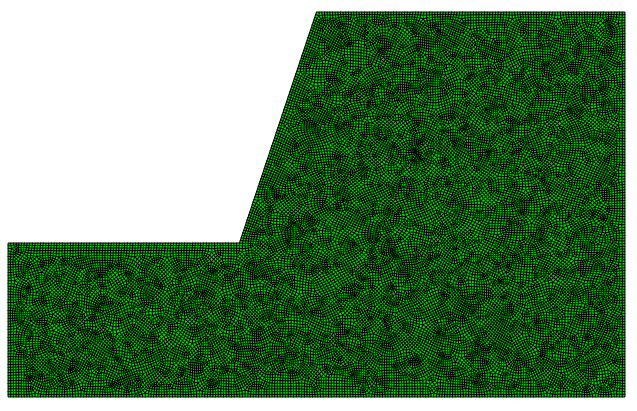
\includegraphics[width=0.6\textwidth]{figures/Chapter5/SlopeMeshNRM}
\caption{{\label{fig:SRM} Mesh for converged Drucker-Prager CDM FEM slope failure simulation
}}
\end{center}
\end{figure}

\begin{figure}[!htb]
\begin{center}
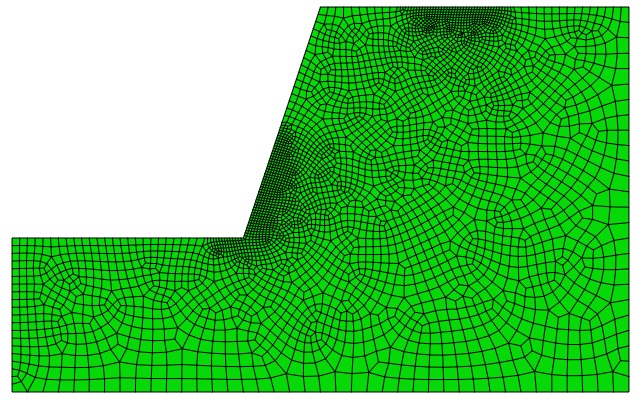
\includegraphics[width=0.6\textwidth]{figures/Chapter5/SlopeMeshSRM}
\caption{{\label{fig:NRM} Selectiverly Refined Mesh (SRM) for Drucker-Prager CDM FEM slope failure simulation.
}}
\end{center}
\end{figure}

\begin{table}[!htb]
\centering
\caption{{Comparison of Computational Time for the \glsentryshort{dns}}}
\label{tab:computation}
\begin{tabularx}{\textwidth}{@{}YYYYY@{}}
\toprule
\textbf{Simulation Type} & \textbf{Continuum Elements} & \textbf{Processor Clock Speed} & \textbf{Slope Failure Load} & \textbf{Computational Time} \\ \midrule
DEM                      & $25,898$                         & $2.20 GHz$                    & $11.2 MPa$                  & $46.5 hr$                  \\
CDM                      & $29,866$                         & $1.80 GHz$                    & $11.5 MPa$                  & $0.65 hr$                  \\
CDM - SRM                      & $3,577$                         & $1.80 GHz$                    & $11.5 MPa$                  & $0.013 hr$                  \\ \bottomrule
\end{tabularx}
\end{table}

The \acrshort{dem} simulation was run serially on a $2.2GHz$ CPU while the \acrshort{cdm} simulation was run serially on a $1.8GHz$ CPU. Despite the \acrshort{cdm} model having more continuum elements than the \acrshort{dem} model, and the \acrshort{cdm} model running on a slower CPU, a decrease in computational time of the \acrshort{dem} simulation from $46.5 hr$ to $0.65 hr$ was observed. Running the \acrshort{cdm} model with a \acrshort{srm} reduces the total computational time to $0.013 hr$, or eight minutes instead of two days. This large increase in computational efficiency with marginal decrease in model accuracy can be immensely useful for large scale geomechanical problems in \acrshort{nfr}. 
